\chapter{Diseño e implementación}
\label{chap:diseño}

El presente capítulo constituye el núcleo técnico de este trabajo. En él se describe de manera exhaustiva el proceso de desarrollo de la plataforma, detallando las decisiones de diseño, el tratamiento de la información y la construcción del \textit{pipeline} predictivo. El objetivo es proporcionar una visión clara y reproducible de cómo se han integrado las diferentes tecnologías para dar solución al problema del pronóstico de aparcamiento mediante \textit{Deep Learning}.

\section{Arquitectura general} 
\label{sec:arquitectura}

Para garantizar la escalabilidad y robustez del sistema, se ha diseñado una arquitectura orientada a los datos, dividida en fases secuenciales que abarcan desde la ingesta hasta la visualización final. La estructura global del proyecto se ilustra en la Figura~\ref{fig:arquitectura}.

\begin{figure}
	\centering
	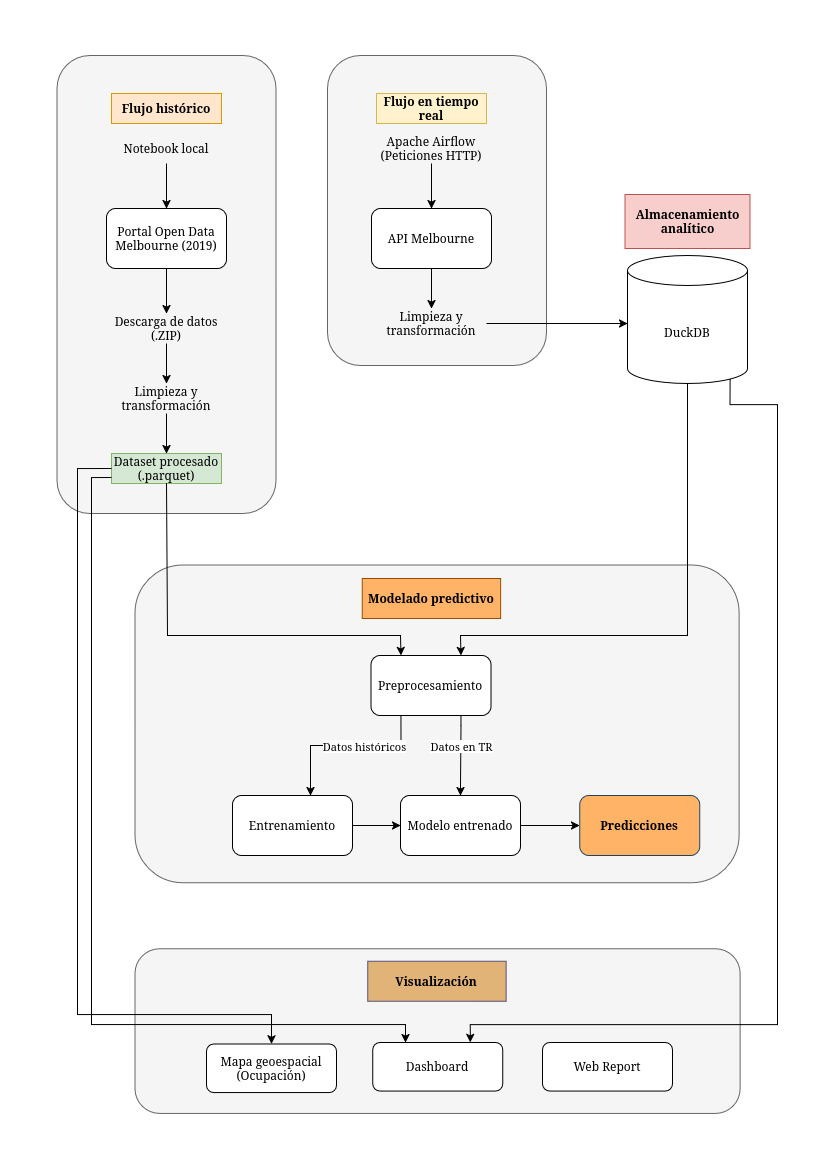
\includegraphics[width=12cm, keepaspectratio]{img/[implem]arquitectura.png}
	\caption{Arquitectura general del pipeline del sistema.}
	\label{fig:arquitectura}
\end{figure}

Tal y como se observa en la Figura~\ref{fig:arquitectura}, el sistema se articula de forma secuencial, dividiendo sus primeras fases (Capas 1 y 2) en dos flujos de trabajo diferenciados según la naturaleza temporal de los datos:
\begin{itemize}
	\item \textbf{Flujo histórico.} Ejecutado de forma local mediante \textit{scripts} de Python, se encarga de la extracción de datos desde el portal de \textit{Open Data} de Melbourne y posteriores transformaciones. Estos datos serán empleados en entrenar el modelo de PyPOTS.
	\item \textbf{Flujo en tiempo real.} Orquestado íntegramente por Apache Airflow, interactúa de forma periódica con la API del Ayuntamiento para obtener los datos en tiempo real, estandarizarlos y mantener el sistema actualizado mediante el almacenamiento en DuckDB. Estos datos serán destinados para realizar la inferencia una vez el modelo ha sido entrenado.
	\item \textbf{Motor de modelado predictivo.} Realiza el entrenamiento con los datos históricos y ejecutar la inferencia para generar las predicciones futuras. 
	\item \textbf{Interfaz de consumo y visualización.} Integración de herramientas específicas según el caso de uso: Grafana para la monitorización de métricas y predicciones, Folium para la representación interactiva de la ocupación geográfica, y Quarto para la web del proyecto.
\end{itemize}



\section{Origen y Comprensión de los Datos}
\label{sec:origen_datos}

El primer paso crítico en cualquier proyecto de analítica predictiva es la adquisición y comprensión del dominio de los datos. Para este trabajo, se ha tomado como base empírica el portal de \textit{Open Data} del Ayuntamiento de Melbourne. 

\subsection{Estructura del \textit{dataset} histórico. Extracción automatizada}
\label{subsec:justificacion}
Para la fase de entrenamiento y experimentación inicial, se recurre al \textit{dataset} histórico estático correspondiente al año 2019. La elección de este año en particular responde a una limitación operativa y contextual importante: debido a las anomalías de movilidad y a los cambios en las políticas de retención de datos durante la pandemia de la COVID-19, los conjuntos de datos posteriores a 2020 presentan vacíos de información o no fueron almacenados de forma persistente. Por tanto, 2019 representa el último ciclo temporal completo y fidedigno de la movilidad urbana ordinaria (incluyendo estacionalidad anual, festividades locales y variaciones estacionales).

Para garantizar la reproducibilidad del entorno de desarrollo y evitar el manejo manual de archivos masivos, la obtención de este conjunto de datos se ha procedimentado mediante un \textit{pipeline} de extracción automatizado en Python. Haciendo uso de librerías nativas como \textit{requests} para peticiones HTTP, se orquestó la conexión al repositorio original para la descarga del archivo comprimido por bloques (\textit{chunks}) para evitar colapsar la memoria RAM.

Una vez finalizada la transferencia, el sistema localiza el archivo (\textit{.zip}), extrae su contenido programáticamente utilizando la librería \textit{zipfile} y almacena los datos tabulares en formato CSV para su posterior procesamiento.

Este conjunto masivo de datos, compuesto por más de 42 millones de registros anuales, presenta un paradigma de almacenamiento orientado a eventos. Cada fila del documento no representa el estado general o agregado de una calle en un intervalo de tiempo dado, sino un evento asíncrono e individual: la llegada (\textit{ArrivalTime}) o la salida (\textit{DepartureTime}) física de un vehículo en un sensor o plaza de aparcamiento específica (\textit{DeviceId} o \textit{Bay ID}), acompañado de su marca temporal exacta.

Esta alta granularidad, si bien es excelente para capturar la realidad del tráfico de agitación plaza por plaza, requiere de un procesamiento intensivo para transformar un registro de eventos asíncronos en una serie temporal regular y estructurada con la que posteriormente poder modelar.

\subsection{Dataset geográfico}
\label{subsec:dataset_geo}
De forma análoga a la obtención del histórico de ocupación, el \textit{pipeline} de extracción se reutiliza para descargar un segundo conjunto de datos: el inventario geográfico de plazas de aparcamiento. Este archivo contiene las coordenadas geográficas precisas (\textit{latitud} y \textit{longitud}) y la descripción del segmento de vía (\textit{road segment description}) de la infraestructura de la ciudad. Su extracción automatizada sigue los mismos principios de eficiencia y reproducibilidad que para el dataset histórico.


\section{Análisis Exploratorio de Datos (EDA)}
\label{sec:eda}

Antes de aplicar cualquier técnica de modelado o de diseñar el esquema de la base de datos analítica, es imperativo realizar un análisis exploratorio de datos. Esta fase persigue un doble objetivo: comprender las distribuciones subyacentes de los datos de movilidad en Melbourne, así como las vairables de interés, e identificar anomalías  en las mediciones físicas de los sensores.

Adicionalmente, se ha identificado que el \textit{dataset} principal, pese a su exhaustividad temporal, carece de componentes geográficas explícitas más allá de identificadores alfanuméricos de las calles. Por tanto, esta fase exploratoria también contempla el enriquecimiento de los datos mediante el cruce con el inventario geográfico de la ciudad, un paso esencial para dotar al análisis de contexto topográfico.

Debido al gran volumen de información, las fases iniciales de diseño del algoritmo de limpieza se han prototipado sobre una muestra representativa de 500.000 filas, un tamaño significativo para obtener conclusiones generalizables al conjunto completo de datos. Esta estrategia permitió agilizar las iteraciones de desarrollo y optimizar el consumo de memoria RAM antes de escalar el proceso al clúster completo.

Tras visualizar las observaciones del \textit{dataset} en formato \textit{DataFrame} de \textit{Pandas}, se realiza una interpretación a alto nivel de las variables presentes, clasificándolas en cuatro categorías principales:

\begin{itemize}
	\item \textbf{Variables temporales:}
	\begin{itemize}
		\item \textit{ArrivalTime} (\texttt{str}): fecha y hora exacta en la que el sensor detectó la llegada del vehículo.
		\item \textit{DepartureTime} (\texttt{str}): fecha y hora exacta en la que el vehículo abandonó la plaza.
		\item \textit{DurationMinutes} (\texttt{str}): tiempo total de estacionamiento (diferencia temporal entre la llegada y la salida).
	\end{itemize}
	
	\item \textbf{Variables de estado:}
	\begin{itemize}
		\item \textit{VehiclePresent} (\texttt{bool}): variable objetivo (\textit{target}). Indica la presencia física de un vehículo sobre el sensor durante ese periodo.
		\item \textit{InViolation} (\texttt{bool}): vndica si el vehículo excedió el tiempo permitido, incurriendo en una infracción.
		\item \textit{Sign} (\texttt{str}) / \textit{SignPlateID} (\texttt{float64}): texto y código identificador de la señal física de tráfico de la calle. Estas variables presentan una alta proporción de valores nulos.
	\end{itemize}
	
	\item \textbf{Identificadores de plazas:}
	\begin{itemize}
		\item \textit{DeviceId} (\texttt{int64}): número de serie electrónico del sensor.
		\item \textit{BayId} (\texttt{int64}): identificador de la plaza de aparcamiento.
		\item \textit{StreetMarker} (\texttt{str}): código alfanumérico identificativo. La tupla formada por (\textit{DeviceId}, \textit{StreetMarker}) constituye una clave única.
	\end{itemize}
	
	\item \textbf{Variables de ubicación:}
	\begin{itemize}
		\item \textit{AreaName} (\texttt{str}): barrio o distrito general al que pertenece la plaza.
		\item \textit{StreetName} (\texttt{str}) / \textit{StreetId} (\texttt{int64}): nombre y código numérico de la calle principal.
		\item \textit{BetweenStreet1} (\texttt{str}) / \textit{BetweenStreet1ID} (\texttt{int64}): primera calle transversal que acota el tramo de estacionamiento.
		\item \textit{BetweenStreet2} (\texttt{str}) / \textit{BetweenStreet2ID} (\texttt{int64}): segunda calle transversal que acota el tramo.
		\item \textit{SideName} (\texttt{str}) / \textit{SideOfStreetCode} (\texttt{str}) / \textit{SideOfStreet} (\texttt{int64}): identificadores de la acera de estacionamiento y su ubicación geográfica (Norte, Sur, Este, Oeste). Existe una equivalencia predefinida entre códigos (1-C, 2-E, 3-N, 4-S, 5-W).
	\end{itemize}
\end{itemize}

\subsection{Transformación y tipificado de variables}
\label{subsec:transformacion}
Los datos brutos presentan inconsistencias de formato que requieren una estandarización previa. En primer lugar, la variable de duración (\textit{DurationMinutes}) fue convertida de cadena de texto a valor numérico de coma flotante (\texttt{float}). Asimismo, las marcas de tiempo (\textit{ArrivalTime} y \textit{DepartureTime}), almacenadas originalmente como texto plano, se transforman a objetos \textit{datetime} nativos, lo cual es indispensable para habilitar la correcta indexación temporal y el posterior remuestreo de la serie.


\subsection{Ingeniería de características (\textit{Feature Engineering})}
\label{subsec:feature_engineering}
Con las variables temporales correctamente tipificadas, se procede a la descomposición de las fechas para extraer componentes estacionales subyacentes. A partir de la fecha de llegada, se generaron tres nuevas características fundamentales:
\begin{itemize}
	\item \textbf{Hora del día (\textit{Hour}):} busca capturar los picos de tráfico laboral diario.
	\item \textbf{Día de la semana (\textit{WeekDay}):} busca entender el comportamiento de la movilidad entre días laborables y fines de semana.
	\item \textbf{Mes del año (\textit{Month}):} ayuda a modelar la macro-estacionalidad, como periodos vacacionales o cambios de estación.
\end{itemize}

\subsection{Análisis descriptivo y visualización}
\label{subsec:visualizacion_eda}
Una vez estandarizado el conjunto de datos y generadas las nuevas variables, se continua con un análisis visual descriptivo para obtener \textit{insights} sobre el comportamiento de la movilidad.

En primer lugar, se analiza la distribución de la variable objetivo binaria (\textit{VehiclePresent}), la cual indica la ocupación física de las plazas. Este paso es crítico para evaluar el balanceo de clases antes de la fase de modelado.

\begin{figure}
	\centering
	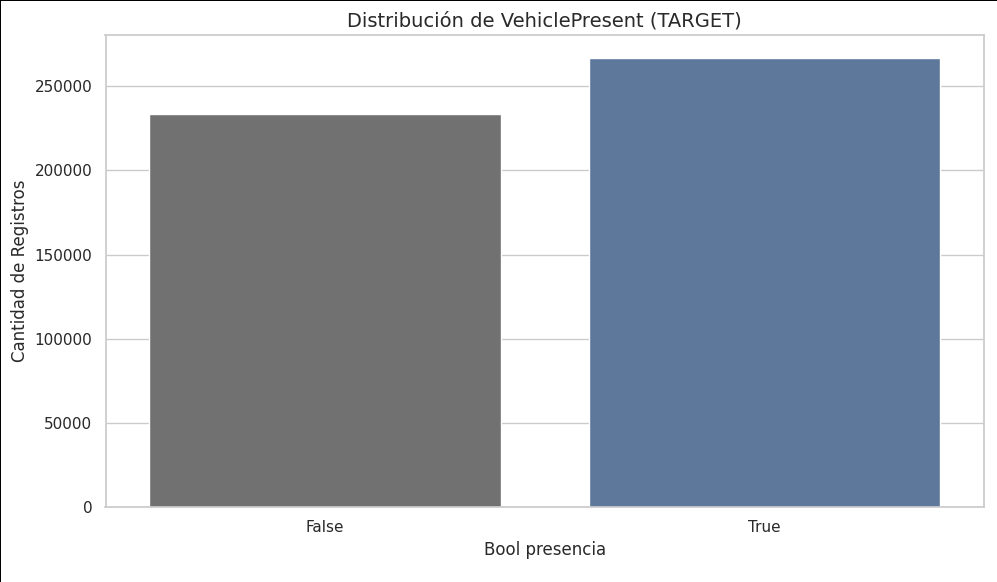
\includegraphics[width=10cm, keepaspectratio]{img/[implem]eda_target.png}
	\caption{Distribución de la variable objetivo (\textit{VehiclePresent}).}
	\label{fig:eda_target}
\end{figure}

Como se aprecia en la Figura~\ref{fig:eda_target}, se evalua la proporción de registros correspondientes a plazas ocupadas frente a plazas libres. En problemas de \textit{Deep Learning}, un desbalanceo severo en la variable a predecir podría inducir a la red neuronal a apostar sistemáticamente por la clase mayoritaria, reduciendo drásticamente su capacidad de generalización. La visualización de esta distribución permite confirmar que no hay un desbalanceo notable, pues ambas clases presentan una representación equilibrada.

Posteriormente, se analiza el volumen de registros de aparcamiento en función de la hora del día, con el fin de identificar los patrones de rotación diarios.

\begin{figure}
	\centering
	
\includegraphics[width=12cm, keepaspectratio]{img/[implem]eda_hours.png}
	\caption{Distribución del volumen de eventos de estacionamiento según la hora del día.}
	\label{fig:eda_hours}
\end{figure}

Tal y como se ilustra en la Figura~\ref{fig:eda_hours}, la movilidad urbana en las plazas sensorizadas presenta un comportamiento fuertemente cíclico y dependiente del horario laboral. Se observa un valle profundo de inactividad durante la madrugada, seguido de un incremento pronunciado a partir de las 08:00 horas. El volumen de eventos se mantiene en niveles máximos durante las horas centrales del día, reflejando la alta rotación comercial y laboral, para finalmente descender de forma paulatina a partir de las 18:00 horas aproximadamente.

Por último, se evalua la distribución espacial de estos eventos para identificar los principales puntos de congestión o \textit{hotspots} de la ciudad. El análisis geográfico representado en la Figura~\ref{fig:eda_hotspots} revela que la demanda de aparcamiento no se distribuye de manera uniforme, sino que se concentra asimétricamente en unas pocas vías principales. Estas calles, que acumulan la mayor densidad de registros, pueden corresponder a arterias de algún distrito central de negocios o a zonas con alta concentración de servicios. Esta información es importante, pues estas zonas serán áreas prioritarias para el modelo predictivo. En relación a las áreas más concurridas destaca \textit{Docklands}, seguida por \textit{Queensberry} y el entorno del \textit{Princes Theatre}.

\begin{figure}
	\centering
	
\includegraphics[width=12cm, keepaspectratio]{img/[implem]eda_hotspots.png}
	\caption{Top de vías o zonas con mayor densidad de registros de aparcamiento (\textit{hotspots}).}
	\label{fig:eda_hotspots}
\end{figure}


\subsection{Integración espacial y georreferenciación de los dispositivos}
\label{subsec:integracion_espacial}

Para dotar al sistema de contexto geoespacial y poder enriquecer la información de entrada de los modelos predictivos, resulta indispensable conocer la ubicación física exacta de cada plaza de aparcamiento. Sin  embargo, el conjunto de datos histórico carece nativamente de las coordenadas geográficas de los sensores. Para solventar esta necesidad, se descarga un conjunto de datos con coordenadas geográficas de los sensores (longitud y latitud), proveniente del ayuntamiento de Melbourne y se realiza un \textit{merge} de datos entre el conocido \textit{dataset} histórico transaccional de 2019 y este nuevo conjunto de datos espaciales.

El proceso de georreferenciación se ejecuta de forma secuencial. En primer lugar, se construye el subconjunto de sensores únicos del histórico a partir de las variables identificativas del dispositivo y su contexto vial  (\texttt{BayId, StreetName}...). A continuación, dado que los identificadores entre ambas fuentes no están estandarizados, se aplica una función de emparejamiento basada en la normalización textual de la toponimia (calle principal y calles transversales), comparando dichas descripciones con los segmentos del conjunto espacial. Cuando existe coincidencia, se asigna al sensor el par de coordenadas de latitud y longitud del segmento correspondiente. Finalmente, se realiza un filtrado para eliminar los sensores no georreferenciados y, posteriormente, se eliminan duplicados de coordenadas para conservar ubicaciones únicas.

El resultado de esta integración es un \textit{dataset} de sensores geolocalizados único. Este subconjunto sirve de base de conocimiento espacial para la clasificación de plazas de parking en función de los puntos de interés desarrollada más adelante (véase la sección~\ref{sec:clasificacion_espacial}), así como para alimentar con contexto geográfico a las distintas arquitecturas de \textit{deep learning}.




%%%%%%%%%%%%%%%%%%%%%%%%%%%%%%%%%%%%%%%%%%%%%%%%%%%%%%%%%%%%%%%%%%%%%%%%%%%%%%%%%%%%%%%%%%%%%%%%%%%%%%%%%
%%%%%%%%%%%%%%%%%%%%%%%%%%%%%%%%%%%%%%%%%%%%%%%%%%%%%%%%%%%%%%%%%%%%%%%%%%%%%%%%%%%%%%%%%%%%%%%%%%%%%%%%%
%%%%%%%%%%%%%%%%%%%%%%%%%%%%%%%%%%%%%%%%%%%%%%%%%%%%%%%%%%%%%%%%%%%%%%%%%%%%%%%%%%%%%%%%%%%%%%%%%%%%%%%%%
\section{Procesamiento de datos para PyPOTS}
\label{subsec:procesamiento_pypots}

Esta sección detalla las transformaciones finales a los datos para la obtención del dataset finalmente utilizado como entrada para los modelos. Este se obtiene al realizar la integración del dataset histórico procesado tras el EDA (con las nuevas variables temporales generadas) con el dataset espacial, también procesado previamente, que contiene los ids sin duplicados de los sensores y su longitud y latitud asociada. 

\subsection{Georreferenciación de observaciones}
El proceso de georreferenciación se ejecuta de forma secuencial. En primer lugar, se construye un diccionario a partir del dataframe espacial, donde cada clave es un identificador de dispositivo (\texttt{DeviceId}) y el valor asociado es un diccionario con las coordenadas 'lat' y 'lon'. Se asignan las coordenadas a cada registro del dataset principal mediante la función map, que busca el identificador de dispositivo en el diccionario y extrae la latitud y longitud correspondientes, de forma que se eliminan aquellos sensores cuyo identificador de dispositivo no se encuentra en el dataframe espacial: el total de observaciones se reduce a 260\,303.

Este nuevo dataset con información enriquecida debe ser adecuado a los requisitos estructurales y matemáticos de la librería PyPOTS como se detalla en las siguientes subsecciones.

\subsection{Generación de \textit{Grid} temporal}
\label{subsec:regularizacion_grid}

El conjunto de datos transaccional original registra los eventos de forma asíncrona; es decir, documenta las llegadas y salidas de los vehículos en instantes de tiempo arbitrarios y variables. Sin embargo, los modelos predictivos de series temporales requieren secuencias de observación regulares, donde la distancia cronológica entre dos fotogramas consecutivos sea estrictamente constante. Para resolver esta discrepancia estructural, se ha implementado un proceso de remuestreo temporal basado en cuadrícula.

En primer lugar, se define un vector temporal continuo con una frecuencia fija de 15 minutos, abarcando desde el primer registro hasta el final de la ventana de estudio. A continuación, se realiza el producto cartesiano entre este vector temporal y los identificadores únicos de los sensores (\texttt{DeviceId}). Esto crea un esqueleto tabular homogéneo donde cada plaza de aparcamiento posee una fila exacta para cada intervalo de 15 minutos, independientemente de si en ese momento concreto realmente ocurrió un evento o no.

Para poblar este esqueleto con el estado real de la calle, se aplica una técnica de cruce por proximidad temporal basada en el último estado conocido (\texttt{merge\_asof}). Este algoritmo evalúa cada marca de tiempo de la cuadrícula (por ejemplo, las 10:15 h) y retrocede cronológicamente hasta encontrar el último evento registrado para ese sensor, propagando su estado de ocupación (\texttt{VehiclePresent}) hacia adelante. Finalmente, se inputan nulos en la secuencia en función de la siguiente restricción: si la marca de tiempo evaluada en la cuadrícula es estrictamente posterior a la hora de salida (\texttt{DepartureTime}) del último vehículo detectado, la ocupación de la plaza pasa a registrarse como nula. 

Esta generación intencionada de valores nulos es un paso de diseño crítico, ya que materializa explícitamente los ``huecos temporales" a imputar en la serie por los algoritmos de imputación de PyPOTS.


\subsection{Codificación cíclica de variables temporales}
\label{subsec:codificacion_ciclica}

Las variables temporales extraídas en la fase de análisis exploratorio, tales como la hora, el día de la semana y el mes, poseen una naturaleza inherentemente cíclica. Si estas características se introducen en la red neuronal como valores enteros secuenciales, el modelo percibirá una distancia matemática irreal; por ejemplo, interpretaría una separación máxima entre las 23:00 y las 00:00, cuando en la realidad cronológica representan instantes consecutivos. Si bien técnicas clásicas de codificación posicional como el \textit{One-Hot Encoding} logran mitigar este sesgo aritmético, se generan vectores ortogonales independientes que destruyen por completo la secuencialidad del tiempo: por ejemplo, se sumiría que un lunes es matemáticamente tan distinto de un martes como de un domingo.

Para preservar la continuidad y el ciclo natural del tiempo sin comprometer la interpretabilidad del modelo, se ha implementado una técnica de codificación cíclica mediante transformaciones trigonométricas. Cada variable temporal se ha descompuesto en dos componentes espaciales continuas proyectadas sobre un círculo unitario. Para cualquier instante temporal $x$, las transformaciones aplicadas se definen como:

$$x_{sin} = \sin\left(\frac{2 \pi \cdot x}{\max(x)}\right)$$
$$x_{cos} = \cos\left(\frac{2 \pi \cdot x}{\max(x)}\right)$$

Gracias a esta proyección, instantes fronterizos como las 23:59 y las 00:01 poseen coordenadas trigonométricas prácticamente idénticas. Esto permite a la red neuronal interpretar correctamente la transición fluida entre ciclos diarios, semanales y mensuales, optimizando el aprendizaje de patrones estacionales sin incrementar desproporcionadamente la dimensionalidad horizontal del conjunto de datos.


\subsection{\textit{Feature Selection}}
\label{subsec:feature_selection}

Como paso final, se a realiza la fase de selección de características. El objetivo primordial de esta etapa consiste en depurar el volumen de información para retener únicamente aquellos atributos que aporten un valor predictivo directo, unívoco y generalizable, y su vez eliminar el ruido y la redundancia que puedan inducir al sobreentrenamiento o penalizar la eficiencia computacional de las redes neuronales. 

Bajo este criterio metodológico, se descartan todas las características de naturaleza textual o administrativa previamente analizados en la fase exploratoria, tales como los nombres descriptivos de las calles, las descripciones de las señales de tráfico o los indicadores de infracción, dado que carecen de propiedades aritméticas explotables por el modelo. Asimismo, identificadores secundarios como los códigos de plaza o de acera se omiten al estar implícitamente representados por el número de serie electrónico del sensor.

\subsection{Consolidación y exportación del conjunto de datos final}
\label{subsec:exportacion_dataset}

Como culminación del flujo de preprocesamiento específico, el conjunto de datos definitivo se exporta en \textit{Parquet}. El \textit{dataset} resultante se caracteriza por ser una matriz de  4\,239\,840 filas y 11 columnas.

El vector de variables que compone formalmente el esquema de este conjunto de datos final está constituido de forma estricta por los siguientes componentes:

\begin{itemize}
	\item \textbf{Identificador del sensor (\texttt{DeviceId}):} clave única que identifica cada dispositivo físico en la red.
	\item \textbf{Marca de tiempo indexada (\texttt{Timestamp}):} registro temporal homogeneizado e indexado en intervalos regulares de 15 minutos.
	\item \textbf{Indicador de ocupación (\texttt{VehiclePresent}):} variable objetivo transformada a \textit{float} para su procesamiento en la red.
	\item \textbf{Coordenadas espaciales de longitud (\texttt{lon}) y latitud (\texttt{lat}):} componentes geográficas que proporcionan el posicionamiento del dispositivo.
	\item \textbf{Transformaciones trigonométricas de la hora (\texttt{Hour\_sin} y \texttt{Hour\_cos}):} par de variables continuas que modelan el ciclo diario.
	\item \textbf{Transformaciones trigonométricas del día (\texttt{WeekDay\_sin} y \texttt{WeekDay\_cos}):} par de variables continuas que modelan el ciclo semanal.
	\item \textbf{Transformaciones trigonométricas del mes (\texttt{Month\_sin} y \texttt{Month\_cos}):} par de variables continuas que modelan el ciclo anual.
\end{itemize}





%%%%%%%%%%%%%%%%%%%%%%%%%%%%%%%%%%%%%%%%%%%%%%%%%%%%%%%%%%%%%%%%%%%%%%%%%%%%%%%%%%%%%%%%%%%%%%%%%%%%%%%%%
%%%%%%%%%%%%%%%%%%%%%%%%%%%%%%%%%%%%%%%%%%%%%%%%%%%%%%%%%%%%%%%%%%%%%%%%%%%%%%%%%%%%%%%%%%%%%%%%%%%%%%%%%
%%%%%%%%%%%%%%%%%%%%%%%%%%%%%%%%%%%%%%%%%%%%%%%%%%%%%%%%%%%%%%%%%%%%%%%%%%%%%%%%%%%%%%%%%%%%%%%%%%%%%%%%%
\section{Modelado de Series Temporales}

El presente capítulo sienta las bases teóricas y matemáticas de las arquitecturas de aprendizaje profundo (\textit{Deep Learning}) seleccionadas para acometer las tareas de imputación y predicción a futuro. A lo largo de las siguientes subsecciones, se desgrana la topología interna de modelos que representan el actual estado del arte en la literatura científica. El estudio inicia con las técnicas de imputación, para posteriormente adentrarse en las arquitecturas predictivas. 


\subsection{Fundamentos Teóricos de los Modelos de Imputación}
\label{sec:theoretical_framework}

Para abordar el desafío matemático de la reconstrucción de series temporales con valores ausentes, el presente trabajo selecciona dos arquitecturas neuronales que representan el estado del arte en sus respectivas familias algorítmicas. En primer lugar, se prueba una aproximación determinista basada en mecanismos de atención (SAITS). Posteriormente, se aplica un enfoque probabilístico fundamentado en modelos de difusión estocástica (CSDI). Ambos algoritmos han demostrado su superioridad teórica y empírica frente a métodos estadísticos tradicionales al ser evaluados en \textit{benchmarks} públicos de gran exigencia, tales como el conjunto de datos médicos PhysioNet-2012 \parencite{silva2012predicting} y el registro meteorológico Beijing PM2.5 \parencite{liang2015assessing}.

\subsubsection{Arquitectura SAITS}

El modelo SAITS (\textit{Self-Attention-based Imputation for Time Series}), propuesto por \textcite{du2023saits}, adapta la exitosa arquitectura \textit{Transformer} \parencite{vaswani2017attention} a las particularidades topológicas de las series temporales con observaciones parciales. A diferencia de las redes recurrentes (RNN) clásicas, propensas al desvanecimiento del gradiente en secuencias largas, SAITS emplea un mecanismo de \textit{self-attention} capaz de capturar dependencias temporales complejas de forma simultánea a lo largo de toda la ventana de observación.

El núcleo matemático de esta arquitectura se fundamenta en un diseño de optimización conjunta mediante bloques de atención con enmascaramiento diagonal. Para procesar la entrada, el sistema proyecta la serie temporal en tres famosas matrices fundamentales: \textit{queries} ($Q$), \textit{keys} ($K$) y \textit{values} ($V$). La relación de importancia entre los distintos instantes temporales se calcula mediante la función de atención multiplicativa escalada:

\begin{equation}
	\text{Attention}(Q, K, V) = \text{softmax}\left(\frac{QK^T}{\sqrt{d_k}}\right)V
\end{equation}

Donde $d_k$ representa la dimensión de las claves. Para prevenir el \textit{data leakage}, SAITS introduce una matriz de enmascaramiento asimétrico que impide a un paso temporal observar su propio valor durante el proceso de autoatención, forzando a la red a estimar dicho valor a partir del contexto circundante. Para prevenir el \textit{data leakage}, SAITS introduce una matriz de enmascaramiento asimétrico (DMSA, \textit{Diagonally-Masked Self-Attention}) que impide a un paso temporal observar su propio valor durante el proceso de autoatención, forzando a la red a estimar dicho valor a partir del contexto circundante. 

A nivel arquitectónico, el modelo no emplea un único bloque, sino una estructura dual en cascada. El primer bloque extrae las representaciones latentes preliminares, mientras que el segundo bloque refina la imputación. A nivel de salida, SAITS conforma un modelo determinista que se entrena mediante una estrategia de optimización conjunta (\textit{joint optimization}). La función de pérdida combina dos objetivos: la Tarea de Reconstrucción Observada (ORT), que asegura la fidelidad frente a los datos reales, y la Tarea de Imputación Enmascarada (MIT), que minimiza el error absoluto (MAE) sobre los valores nulos artificialmente inyectados durante el entrenamiento. Esta combinación garantiza que el tensor finalmente emitido mantenga tanto la coherencia local como la dinámica global de la serie.

\subsubsection{Arquitectura CSDI}

Por su parte, el algoritmo CSDI (\textit{Conditional Score-based Diffusion Models for Probabilistic Time Series Imputation}), introducido por \textcite{tashiro2021csdi}, aborda el problema de la imputación desde una perspectiva probabilística y generativa. Al basarse en los Modelos Probabilísticos de Difusión de Eliminación de Ruido (DDPM) \parencite{ho2020denoising}, esta arquitectura no busca predecir un valor único, sino modelar la distribución de probabilidad completa de los datos ausentes condicionada a las observaciones existentes.

El funcionamiento interno de CSDI se divide en dos procesos estocásticos de tipo cadena de Markov. El primer paso, denominado proceso de difusión hacia adelante (\textit{forward process}), consiste en inyectar ruido gaussiano de forma iterativa y gradual sobre los datos originales durante $T$ pasos continuos, hasta transformar la serie temporal en ruido blanco puro. La distribución de transición para un paso temporal $t$ se define como:

\begin{equation}
	q(x_t | x_{t-1}) = \mathcal{N}(x_t; \sqrt{1 - \beta_t} x_{t-1}, \beta_t \mathbf{I})
\end{equation}

Donde $\beta_t$ controla la varianza del ruido inyectado. El segundo paso, conocido como proceso inverso (\textit{reverse process}), entrena a una red neuronal paramétrica para aproximar la \textit{score function} y revertir el ruido paso a paso. En el contexto específico de CSDI, este proceso inverso se encuentra fuertemente condicionado por los valores observados y por la inyección de \textit{embeddings} que codifican el instante de tiempo y la característica multivariante. Para procesar dicha información, la red paramétrica interna implementa un mecanismo de atención bidimensional: una capa de atención temporal que modela las dependencias cronológicas, seguida de una capa de atención de características (\textit{feature attention}) que captura las correlaciones espaciales entre las distintas variables del sistema (ej. relaciones entre diferentes sensores o variables meteorológicas).

Al concluir la inferencia, el modelo probabilístico no devuelve un único tensor, sino una distribución de posibles trayectorias válidas para la serie temporal. Para someter este resultado a una métrica de precisión geométrica como el MAE o el MSE, el sistema debe extraer un valor puntual representativo al calcular la media o la mediana sobre el conjunto de trayectorias generadas, lo que dota a la predicción final de una gran robustez frente a anomalías locales.



\subsection{Fundamentos Teóricos de los Modelos de Predicción}
\label{sec:theoretical_framework_forecasting}

A diferencia de la imputación, que busca estimar valores ausentes mediante el contexto global, la predicción consiste en la generación de secuencias futuras a partir de una ventana de observación histórica. Para ello, se han seleccionado tres arquitecturas representativas de los paradigmas actuales de \textit{Deep Learning}: la descomposición lineal, el mecanismo de atención pura y la convolución isométrica.

\subsubsection{Arquitectura DLinear}

El modelo DLinear, propuesto por \textcite{zeng2023are}, desafía la hegemonía de las arquitecturas complejas basadas en \textit{Transformers} mediante un enfoque de descomposición de series temporales. Su diseño se fundamenta en la premisa de que gran parte de la señal temporal puede explicarse mediante dos componentes básicos: una tendencia a largo plazo y una estacionalidad cíclica.

DLinear descompone la serie de entrada $X$ en dos flujos:
\begin{equation}
	X_{\text{trend}} = \text{MovingAverage}(X), \quad X_{\text{seasonal}} = X - X_{\text{trend}}
\end{equation}

Donde la tendencia ($X_{\text{trend}}$) se extrae mediante un filtro de media móvil undimensional. Posteriormente, cada componente es procesado de manera independiente mediante redes neuronales de una sola capa lineal (\textit{fully connected}). A diferencia de los modelos basados en atención, que son invariantes a la permutación y requieren codificaciones posicionales artificiales, las capas lineales de DLinear mapean directamente la serie histórica completa hacia la ventana de predicción. Esta simplicidad no solo reduce drásticamente el coste computacional y el riesgo de sobreajuste (\textit{overfitting}), sino que preserva intrínsecamente el orden semántico del tiempo, lo que permite al modelo extrapolar tendencias a largo plazo con un número mínimo de parámetros. La salida final se obtiene mediante la suma de las proyecciones de ambos componentes.

\subsubsection{Arquitectura Transformer}

La arquitectura \textit{Transformer}, extrapolada del procesamiento de lenguaje natural \parencite{vaswani2017attention}, ha sido adaptada al \textit{forecasting} mediante un esquema \textit{encoder-decoder}. En este dominio, el \textit{encoder} procesa la serie temporal de entrada para generar representaciones latentes, mientras que el \textit{decoder} genera la secuencia futura. 

El componente central es el mecanismo de \textit{self-attention}, que permite a cada paso temporal "atender" a cualquier otro punto de la serie, capturando dependencias de largo alcance que las redes recurrentes ignoran. Matemáticamente, el modelo mapea la secuencia de entrada $S_{\text{input}}$ hacia un espacio de alta dimensión, con múltiples proyecciones en paralelo (\textit{multi-head attention}) para capturar diversas dinámicas temporales (e.g ciclos diarios y semanales). Sin embargo, a pesar de su indiscutible éxito en el dominio discreto del procesamiento de lenguaje, la aplicación del Transformer estándar a series temporales continuas presenta retos significativos. Por un lado, su complejidad temporal cuadrática $O(L^2)$ respecto a la longitud de la secuencia de entrada ($L$) restringe drásticamente la capacidad de procesar ventanas históricas extensas. Por otro lado, la atención basada en puntos (\textit{point-wise attention}) es altamente susceptible a anomalías y ruido sensórico de alta frecuencia, lo que a menudo dificulta la extracción de patrones globales estables en el análisis del tráfico urbano a largo plazo.

\subsubsection{Arquitectura MICN}

El modelo MICN (\textit{Multi-scale Isometric Convolutional Network}), introducido por \textcite{wang2023micn}, propone una alternativa eficiente a los \textit{Transformers} mediante la implementación de convoluciones isométricas. Esta arquitectura reconoce que las series temporales poseen patrones tanto locales como globales y que tratar ambos niveles con un mismo filtro es subóptimo.

A nivel estructural, MICN integra un diseño jerárquico basado en el submuestreo a múltiples escalas. En cada bloque de la red, la señal se bifurca para ser procesada simultáneamente por dos mecanismos de convolución unidimensional. El primer mecanismo extrae características locales granulares (cambios a corto plazo), mientras que el segundo mecanismo, basado en convoluciones isométricas, amplía dinámicamente el campo receptivo para modelar el contexto global (tendencias a largo plazo). La característica ``isométrica" asegura que la red mantenga la alineación posicional de la señal, mitigando la pérdida de resolución espacial inherente al \textit{pooling} estándar. Al fusionar la visión local y global mediante capas de retroalimentación cruzada, MICN logra capturar correlaciones temporales complejas con una complejidad computacional lineal $O(L)$, erigiéndose como una solución más ligera y robusta que la autoatención pura para horizontes predictivos cortos y medios.


\subsection{Modelos de Referencia. \textit{Baselines}}
\label{sec:baselines}

Para garantizar la validez científica de los resultados, resulta imprescindible establecer un marco de referencia empírico. Se incorporan \textit{baselines} que permitan establecer una cota inferior de rendimiento aceptable para cada tarea.

\subsubsection{Baselines de Imputación: Inercia y Tendencia Central}

En el contexto específico de imputación de series temporales, el método determinista de referencia por excelencia es la propagación de la última observación válida (LOCF, por sus siglas en inglés, \textit{Last Observation Carried Forward}) \parencite{little2019statistical}. Esta heurística asume que el estado dinámico del sistema tiende a permanecer estático en el corto plazo, hipótesis que cobra especial relevancia técnica en el dominio de los sensores de estacionamiento, donde la ocupación de una plaza suele mantenerse constante durante intervalos temporales. 

Junto al algoritmo LOCF, se desarrollan métodos de imputación por medidas de tendencia central, concretamente la Media Global. Mientras que LOCF establece la cota de rendimiento basada en la inercia temporal, las aproximaciones estadísticas unidimensionales rellenan los valores ausentes al calcular el promedio histórico de la variable, al ignorar por completo la secuencia cronológica \parencite{moritz2015imputeTS}.

\subsubsection{Baseline de Predicción: El límite de la linealidad (DLinear)}

En el ámbito de la predicción futura, la selección del modelo de referencia responde a una necesidad metodológica propia de la investigación contemporánea en Inteligencia Artificial. Durante los últimos años, la proliferación de arquitecturas tipo \textit{Transformers} ha eclipsado a los métodos paramétricos tradicionales bajo la premisa de que las relaciones no lineales profundas son necesarias para predecir el futuro. Sin embargo, estudios recientes \parencite{zeng2023are} han cuestionado severamente esta tendencia. Los autores demuestran que los mecanismos de autoatención son inherentemente invariantes a la permutación, lo que provoca una pérdida de información sobre el orden temporal continuo de la señal. En consecuencia, estas redes altamente parametrizadas tienden a sobreajustarse y degradar el modelado de dependencias temporales estrictas frente a enfoques lineales simples que preservan intacta la cronología de los datos.

Por este motivo, se establece a DLinear no solo como un modelo predictivo objeto de estudio, sino conceptualmente como el \textit{baseline} estructural frente al resto de arquitecturas avanzadas. Al reducir el proceso de inferencia a una mera extracción de tendencia por media móvil y un mapeo directo mediante una capa lineal, DLinear carece de la capacidad de extraer características complejas a múltiples escalas, al contrario que MICN, o de modelar interacciones cruzadas complejas, como sí hace la arquitectura Transformer.





\section{Implementación del Flujo de Entrenamiento y Predicción}
\label{flujo_imput_pred}

El presente capítulo detalla la arquitectura de software modular empleada para la ejecución automatizada de los modelos PyPOTS.En los apartados sucesivos se desgrana el tratamiento aplicado a las series temporales, el diseño del espacio de búsqueda, los mecanismos de entrenamiento y monitorización, y el marco de métricas establecido para evaluar el rendimiento predictivo final frente a los modelos estadísticos de referencia.

\subsection{Preparación y Enmascaramiento de Datos}
\label{sec:data_preparation}

De forma previa a la instanciación de cualquier arquitectura neuronal, el sistema debe adecuar la información en bruto para hacerla compatible con ciertos requerimientos matemáticos. El proceso de ingesta inicia al cargar el conjunto de datos estructurado en formato \textit{Parquet}. Con el objetivo de obtener unos tiempos de experimentación razonables con los recursos computacionales disponibles, se selecciona un subconjunto correspondiente a una fracción de los sensores IoT disponibles en la red urbana. Para asegurar la reproducibilidad estricta de todos los experimentos y aislar la varianza paramétrica, este muestreo se realiza tras fijar una semilla pseudoaleatoria constante. 

A diferencia de otros problemas clásicos de aprendizaje automático, dividir series temporales exige respetar de forma estricta el orden cronológico. Una partición puramente aleatoria provocaría \textit{data leakage} por lo que se segmenta el conjunto de datos en base a umbrales temporales exactos: el 60\% inicial de los registros históricos conforma el conjunto de entrenamiento (\textit{train}), el 20\% intermedio se destina a la validación durante la optimización paramétrica (\textit{validation}), y el 20\% final se reserva de manera exclusiva para la evaluación definitiva del rendimiento predictivo (\textit{test}).

Para transformar la serie temporal continua en una estructura espacial discreta que sea compatible con el entrenamiento por lotes de las redes neuronales, el componente de carga de datos implementa una técnica de ventanas deslizantes. Esta técnica se aplica diferentemente en función de la tarea objetivo:

\begin{itemize}
	\item \textbf{Imputación.} El sistema extrae secuencias continuas avanzando un paso temporal por iteración. Para un tamaño de ventana $W$, el tensor resultante captura únicamente el contexto histórico local para ser reconstruido.
	\item \textbf{Forecasting.} La extracción se vuelve dual. Por cada iteración, el algoritmo recorta una matriz histórica $X$ de tamaño $W$ y, de forma contigua, extrae una matriz objetivo futura $Y$ de longitud equivalente al horizonte predictivo predefinido. Esta separación estricta garantiza que el modelo proyecte el futuro sin contaminarse de los valores objetivo.
\end{itemize}

El resultado final de esta operación geométrica es la generación de tensores tsridimensionales de dimensiones $(N, W, F)$, donde $N$ representa el número total de muestras extraídas de la ventana deslizante, $W$ la profundidad temporal y $F$ el número de características multivariantes seleccionadas (presencia de vehículos, coordenadas geoespaciales, componentes trigonométricas...).

Finalmente, la evaluación cuantitativa de los modelos de imputación exige disponer de una verdad fundamental (\textit{ground truth}) para medir el margen de error con precisión matemática. Dado que el objetivo primordial consiste en predecir vacíos en la seria temporal, resulta indispensable ocultar de forma artificial una fracción de los datos reales durante la fase de entrenamiento.

Para los conjuntos de validación y prueba, el algoritmo identifica las coordenadas exactas de los valores correctamente observados y procede a enmascarar de forma estocástica un porcentaje del 15\% de ellos con \texttt{NaNs}. Desde el punto de vista estadístico, este procedimiento genera un patrón de ausencia de tipo \textit{Missing Completely At Random} (MCAR) \cite{rubin1976inference}, ya que la probabilidad de que una observación sea ocultada es totalmente independiente del estado del sistema. Esta estrategia matricial permite entregar una señal degradada a la red neuronal, mientras retiene la matriz original intacta. De este modo, el sistema analítico puede cuantificar el error absoluto y cuadrático de forma exclusiva sobre aquellas coordenadas espaciotemporales donde se introdujo el vacío artificial, lo cual garantiza un marco de medición objetivo e inalterable.

\subsection{Definición de Métricas de Evaluación}
\label{sec:metrics}

Para cuantificar el grado de precisión geométrica de las arquitecturas neuronales, resulta necesario establecer un marco matemático de evaluación robusto. Tanto en el contexto de la imputación de series temporales como en la predicción de las mismas, el sistema se enfrenta a un problema de minimización: cuanto menores resulten los valores de las métricas de error, mayor será el rendimiento del modelo. Este principio rige de igual manera en la fase de validación, para la selección de hiperparámetros y parada temprana (\textit{Early Stopping}), y en la fase de evaluación final en \textit{test}.

La discrepancia entre los valores reales y las estimaciones generadas por la red neuronal se evalúa aislando la señal objetivo. En las tareas de imputación, el cálculo se restringe de forma exclusiva a las coordenadas donde se introdujo ruido sintético; mientras que, en la predicción, se evalúa sobre la totalidad de la ventana futura inexplorada. Si se define $n$ como el número total de datos a evaluar, $y_i$ como el valor real correspondiente a la verdad fundamental, y $\hat{y}_i$ como la predicción generada por el modelo, el rendimiento del sistema se analiza a través de tres indicadores estandarizados.

La primera métrica implementada es el Error Absoluto Medio (MAE). Esta función calcula el promedio de las diferencias absolutas entre las predicciones y las observaciones empíricas. El MAE proporciona una medida lineal del error, lo que otorga el mismo peso a todas las desviaciones, independientemente de su magnitud, y facilita la interpretación directa en la misma escala que los datos originales. Matemáticamente, se expresa como:

\begin{equation}
	\text{MAE} = \frac{1}{n} \sum_{i=1}^{n} | y_i - \hat{y}_i |
\end{equation}

Para penalizar de forma severa las discrepancias de gran magnitud, el sistema calcula el Error Cuadrático Medio (MSE). A diferencia de la métrica anterior, el MSE eleva al cuadrado la diferencia entre el valor estimado y el valor real antes de promediar los resultados. Esta propiedad matemática resulta fundamental para detectar y mitigar predicciones extremas u \textit{outliers} generados por el modelo, por lo que se establece como la métrica principal para guiar el mecanismo de parada temprana durante el entrenamiento. Su formulación es la siguiente:

\begin{equation}
	\text{MSE} = \frac{1}{n} \sum_{i=1}^{n} (y_i - \hat{y}_i)^2
\end{equation}

Finalmente, para preservar la alta sensibilidad ante errores pronunciados del MSE, pero retornar el resultado a las unidades originales de la variable estudiada, se calcula la Raíz del Error Cuadrático Medio (RMSE). Esta métrica permite interpretar la desviación estándar de los residuos de las predicciones, lo que resulta de gran utilidad para comparar el rendimiento final de distintas familias algorítmicas en la fase de prueba. Su cálculo se obtiene al aplicar la raíz cuadrada a la función anterior:

\begin{equation}
	\text{RMSE} = \sqrt{\frac{1}{n} \sum_{i=1}^{n} (y_i - \hat{y}_i)^2}
\end{equation}


\subsection{Espacios de Búsqueda y Justificación Paramétrica}
\label{sec:hyperparameters_space}

Dada la alta complejidad interna de los modelos empleados, se considera la realización de una optimización de hiperparámetros para refinar su comportamiento. En lugar de evaluar permutaciones infinitas, el sistema fusiona un conjunto de parámetros estructurales estáticos con un espacio de búsqueda dinámico acotado. Para evitar \textit{overfitting}, el número de épocas no se somete a exploración; se establece un límite superior conservador (entre 20 y 30 iteraciones dependiendo de la tarea) acoplado a un mecanismo de parada temprana con una paciencia estricta de 2 épocas, configurado para almacenar de forma exclusiva los pesos obtenidos por los modelos con menor MSE en validación.

Para dotar a esta búsqueda de la mejor configuraciónd e hiperparámetros de rigor estadístico, el número de iteraciones ejecutadas se fundamenta probabilísticamente. Matemáticamente, la probabilidad $P$ de encontrar al menos una configuración paramétrica que se sitúe en el $10\%$ superior del espacio de rendimiento tras $n$ iteraciones independientes se define como:

$$ P = 1 - (1 - 0.1)^n $$

Para garantizar un nivel de confianza empírica superior al $90\%$ ($P > 0.90$), se requiere resolver la inecuación, lo que arroja un mínimo de $n = 22$ iteraciones. Por consiguiente, el diseño experimental se establece en 22 iteraciones como estándar metodológico para todas las arquitecturas evaluadas. 


\subsubsection{Configuraciones para tareas de Imputación}

Para el modelo SAITS, el espacio de configuración final resultante de la fusión paramétrica se define como sigue:

\begin{listing}[H]
	\caption{Espacio de búsqueda y configuración base para la arquitectura SAITS.}
	\label{lst:json_saits}
	\begin{minted}[frame=lines, framesep=2mm, baselinestretch=1.2, fontsize=\footnotesize, breaklines, obeytabs=true, tabsize=4]{json}
		{
			"epochs": 20,
			"patience": 2,
			"model_saving_strategy": "best",
			"window_size": [48, 96],
			"batch_size": [32, 64],
			"lr": {"distribution": "loguniform", "min": 0.0001, "max": 0.005},
			"n_layers": [2, 3],
			"d_model": [128, 256],
			"n_heads": [2, 4],
			"dropout": [0.1, 0.2]
		}
	\end{minted}
\end{listing}

La selección teórica de estos umbrales responde a las particularidades topológicas de las series temporales. A diferencia de los modelos de procesamiento de lenguaje natural, las redes aplicadas a predicción secuencial tienden a memorizar el ruido local si se diseñan con excesiva profundidad \parencite{zeng2023are}. Por este motivo, el número de capas se restringe deliberadamente a un rango superficial de entre 2 y 3 bloques. Asimismo, se opta por explorar tamaños de ventana temporal de 48 y 96 pasos, dimensiones diseñadas de forma específica para capturar ciclos locales (12 y 24 horas) en los sensores de tráfico urbano. En consonancia con la literatura original \parencite{vaswani2017attention}, la dimensionalidad latente se establece en potencias de 2 (128, 256) estrictamente divisibles por el número de cabezales de atención. La tasa de aprendizaje se explora bajo una distribución log-uniforme para permitir al optimizador muestrear magnitudes de ajuste fino con mayor frecuencia.

Por otro lado, la arquitectura probabilística de difusión (CSDI) presenta requerimientos computacionales notablemente distintos:

\begin{listing}[H]
	\caption{Espacio de búsqueda y configuración base para la arquitectura CSDI.}
	\label{lst:json_csdi}
	\begin{minted}[frame=lines, framesep=2mm, baselinestretch=1.2, fontsize=\footnotesize, breaklines, obeytabs=true, tabsize=4]{json}
		{
			"epochs": 20,
			"patience": 2,
			"model_saving_strategy": "best",
			"target_strategy": "random",
			"n_diffusion_steps": 30,
			"d_time_embedding": 128,
			"d_feature_embedding": 128,
			"d_diffusion_embedding": 128,
			"window_size": [48, 96],
			"batch_size": [64, 128],
			"lr": {"distribution": "loguniform", "min": 0.0001, "max": 0.005},
			"n_layers": [3, 4],
			"n_channels": [64, 128],
			"n_heads": [2, 4],
			"dropout": [0.1, 0.2]
		}
	\end{minted}
\end{listing}

En este segundo escenario, las variables exclusivas del proceso estocástico no se someten a exploración aleatoria para evitar obtener configuraciones de parametros entrenables enormes. Los \textit{embeddings} se fijan en 128 dimensiones al seguir de forma rigurosa las especificaciones empíricas recomendadas por los autores originales \parencite{tashiro2021csdi}. Resulta crítico destacar el redimensionamiento de dos parámetros clave para viabilizar el entrenamiento: los pasos de difusión se acotan a 30 para obtener tiempos de inferencia razonables y el tamaño de lote se eleva a un rango de entre 64 y 128 muestras para maximizar la paralelización en la tarjeta gráfica.

\subsubsection{Configuraciones para Tareas de Predicción}

A diferencia de la imputación local, el abordaje del problema predictivo exige a las redes neuronales asimilar un contexto histórico mucho más extenso. En problemas de predicción de series temporales multivariantes, resulta imperativo establecer una relación óptima entre la longitud de la ventana de observación histórica ($L_{in}$) y el horizonte de predicción objetivo ($L_{out}$). 

En la presente investigación, para el escenario predictivo a corto plazo (24 horas), se ha adoptado la estrategia heurística estándar de la literatura en la que la ventana de entrada se establece como el doble del horizonte temporal. Dado que la red IoT registra eventos cada 15 minutos, el horizonte de 24 horas equivale a 96 pasos ($L_{out}^{24h} = 96$) y consecuentemente requiere un contexto de entrada de 192 pasos ($L_{in}^{24h} = 192$). Para el escenario a medio plazo (48 horas), preservar esta proporcionalidad estricta implica procesar un horizonte de 192 pasos a partir de un bloque histórico de 384 pasos ($L_{in}^{48h} = 384$).

Para acometer esta tarea a gran escala, el modelo DLinear define su espacio de búsqueda de hiperparámetros como sigue:

\begin{listing}[H]
	\caption{Espacio de búsqueda y configuración base para la arquitectura DLinear.}
	\label{lst:json_dlinear}
	\begin{minted}[frame=lines, framesep=2mm, baselinestretch=1.2, fontsize=\footnotesize, breaklines, obeytabs=true, tabsize=4]{json}
		{
			"epochs": 30,
			"patience": 2,
			"model_saving_strategy": "best",
			"window_size": [192, 384],
			"batch_size": [64, 128, 256],
			"lr": {"distribution": "loguniform", "min": 0.0005, "max": 0.01},
			"moving_avg_window_size": [25, 51, 99, 149]
		}
	\end{minted}
\end{listing}

Dada la extrema ligereza matemática de sus capas completamente conectadas, el algoritmo DLinear admite tolerancias elevadas en la ingesta de datos. Esto permite que el tamaño de lote se escale hasta 256 muestras por iteración en ambos horizontes sin provocar desbordamientos de VRAM. El parámetro crítico de esta arquitectura radica en su núcleo de descomposición, una técnica de filtrado adoptada de arquitecturas predecesoras como Autoformer \parencite{wu2021autoformer}: \textbf{la ventana de media móvil}. Se exploran dimensiones impares para garantizar un filtrado central simétrico, evitando desfases cronológicos. Es imperativo señalar la bifurcación estructural dependiente del horizonte: para el escenario de 24 horas (\texttt{window\_size = 192}), el espacio exploró núcleos más cerrados (\texttt{[25, 51, 99]}), mientras que para el escenario de 48 horas (\texttt{window\_size = 384}), el espacio debió ensancharse (\texttt{[51, 99, 149]}) para evitar que un filtro demasiado pequeño resultara incapaz de capturar la macrotendencia en un vector histórico del doble de longitud.

En contraste, la parametrización de la arquitectura Transformer exige un diseño exploratorio mucho más conservador, debido a su complejidad algorítmica cuadrática:

\begin{listing}[H]
	\caption{Espacio de búsqueda y configuración base para la arquitectura Transformer.}
	\label{lst:json_transformer}
	\begin{minted}[frame=lines, framesep=2mm, baselinestretch=1.2, fontsize=\footnotesize, breaklines, obeytabs=true, tabsize=4]{json}
		{
			"epochs": 20,
			"patience": 2,
			"model_saving_strategy": "best",
			"window_size": [192, 384],
			"batch_size": [16, 32, 64, 128],
			"lr": {"distribution": "loguniform", "min": 0.0001, "max": 0.005},
			"n_layers": [2, 3],
			"d_model": [128, 256],
			"n_heads": [2, 4, 8],
			"dropout": [0.1, 0.2]
		}
	\end{minted}
\end{listing}

Al someter el mecanismo de autoatención a secuencias continuas de hasta 384 pasos, el consumo de memoria escala exponencialmente debido a la complejidad espacial $O(L^2)$ del \textit{self-attention} estándar, una limitación crítica ampliamente documentada en el análisis de series temporales largas \parencite{zhou2021informer}. Esta limitación requiere una adaptación asimétrica del espacio de búsqueda en función del tamaño de ventana. Mientras que para la ventana de 192 pasos la tarjeta gráfica admite tamaños de lote convencionales (\texttt{batch\_size} entre 32 y 128 secuencias), al procesar la ventana de 384 pasos el lote máximo admitido antes del desbordamiento de memoria se desploma a 64, por lo que se incluye exploración en rangos mínimos operativos de hasta 16 secuencias. En ambas configuraciones, el espacio prioriza la diversificación de la dimensionalidad latente y la multiplicidad de cabezales, con el objetivo de dotar al modelo de la máxima capacidad de abstracción bajo estas restricciones de hardware.

Finalmente, fiel a los preceptos teóricos que la postulan como una alternativa espacialmente más ligera que los Transformers \parencite{wang2023micn}, se establece la configuración de la arquitectura convolucional isométrica (MICN):

\begin{listing}[H]
	\caption{Espacio de búsqueda y configuración base para la arquitectura MICN.}
	\label{lst:json_micn}
	\begin{minted}[frame=lines, framesep=2mm, baselinestretch=1.2, fontsize=\footnotesize, breaklines, obeytabs=true, tabsize=4]{json}
		{
			"epochs": 20,
			"patience": 2,
			"model_saving_strategy": "best",
			"conv_kernel": [7, 9],
			"window_size": [192],
			"batch_size": [32, 64, 128],
			"lr": {"distribution": "loguniform", "min": 0.0005, "max": 0.005},
			"n_layers": [1, 2],
			"d_model": [64, 128],
			"dropout": [0.1, 0.2]
		}
	\end{minted}
\end{listing}

Como se documenta en el espacio paramétrico (\texttt{window\_size = 192}), el diseño experimental de MICN rompe con la proporcionalidad estricta descrita al inicio de la sección, manteniendo un espacio de búsqueda unificado y estático para ambos horizontes predictivos (24 y 48 horas). La literatura empírica demuestra que el escalado lineal no siempre es computacionalmente viable. En arquitecturas basadas en convoluciones multiescala y submuestreo jerárquico como MICN, inyectar ventanas de 384 pasos provoca el colapso del campo receptivo, derivando en inestabilidades matriciales donde el tamaño del filtro supera la dimensión de la señal comprimida en las capas profundas.

Por este motivo estructural, para el escenario de 48 horas se ha optado metodológicamente por igualar la ventana de entrada al horizonte de predicción ($L_{in}^{48h} = L_{out}^{48h} = 192$). Esta decisión garantiza la estabilidad numérica necesitada para las convoluciones de la red.

Esta homogeneidad espacial de entrada, combinada con la complejidad computacional lineal $O(L)$ de la arquitectura, permite explorar tamaños de lote consistentes y amplios (\texttt{batch\_size} entre 32 y 128 secuencias) en ambas pruebas sin riesgo de desbordamiento. Para preservar el propósito fundacional de sus creadores, el espacio acota deliberadamente la dimensionalidad latente (\texttt{d\_model} en 64 y 128) y restringe la profundidad a redes superficiales (\texttt{n\_layers} a 1 o 2 bloques). Finalmente, su núcleo de extracción se apoya en una parametrización convolucional estática (\texttt{conv\_kernel: [7, 9]}), donde el filtro menor captura las dependencias locales de alta frecuencia y el superior modela las macrotendencias globales de la señal.


\subsection{Orquestación y Automatización del Flujo}
\label{sec:main_orchestrator}

El proceso de entrenamiento se automatiza completamente mediante una arquitectura de software diseñada para aislar la complejidad matemática y maximizar el uso de los recursos computacionales de forma desatendida. Para se desarrollan \textit{scripts} de \textit{Bash} para ejecutar secuencialmente las diferentes iteraciones de los modelos de imputación y predicción. Estos archivos actúan como una capa de ejecución superior del entorno: se inicializa el entorno virtual, se inyecta las variables necesarias para el enlace correcto de los módulos y se lanzan los comandos de ejecución del pipeline de optimización. Esta aproximación de cola secuencial garantiza la estabilidad física de los recursos y permite ejecutar ciclos completos de optimización de manera ininterrumpida


Una vez el \textit{script} inicia la ejecución de un modelo, el ciclo de vida algorítmico sigue un esquema lógico iterativo, el cual se ilustra detalladamente en la Figura \ref{fig:flujo_orquestador}.

\begin{figure}[htbp]
	\centering
	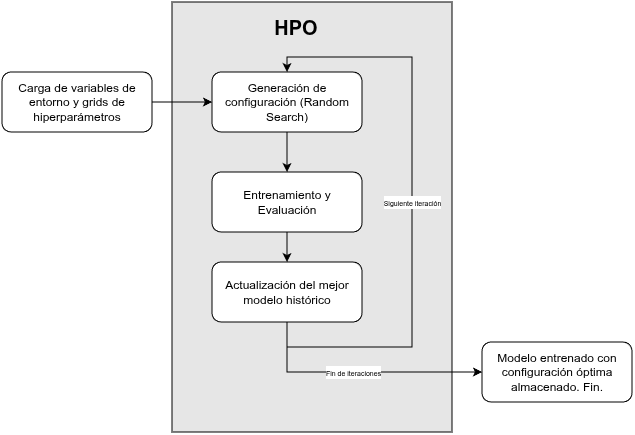
\includegraphics[width=0.85\textwidth, keepaspectratio]{img/[implem]flujo_hpo_pypots.png}
	\caption{\textit{High Performance Optimization}: flujo lógico de optimización de hiperparámetros.}
	\label{fig:flujo_orquestador}
\end{figure}

El sistema orbita en torno a un orquestador central que gestiona este flujo. El proceso se divide en las siguientes etapas fundamentales:

\begin{enumerate}
	\item \textbf{Carga de entorno e inicialización:} El sistema procesa los diccionarios de hiperparámetros y prepara los espacios de búsqueda dinámica definidos en la Sección \ref{sec:hyperparameters_space}.
	\item \textbf{Generación de configuración.} En cada iteración, el algoritmo genera una configuración paramétrica única mediante un muestreo probabilístico (\textit{Random Search}). Si el espacio requiere una distribución log-uniforme (como la tasa de aprendizaje), se transforma el intervalo matemáticamente para extraer un valor continuo aleatorio.
	\item \textbf{Entrenamiento y Evaluación.} El orquestador delega el flujo en el módulo de entrenamiento, el cual inicializa la red neuronal. Durante esta fase, se evalúa la capacidad de generalización del modelo utilizando los criterios de validación y las métricas de error previamente definidas (ver Sección \ref{sec:metrics}). Además, para dotar al proceso de robustez, toda invocación se encapsula en un bloque lógico de control de excepciones, de forma que se contemplen posibles errores de CUDA y/o GPU. Si una iteración falla, se libera la caché de la GPU y se avanza a la siguiente iteración sin interrumpir el flujo global.
	\item \textbf{Actualización del mejor modelo histórico.} Tras evaluar la iteración, el orquestador compara la métrica de error resultante con el mejor registro histórico. Si la configuración actual supera a la anterior, se retienen en memoria y en disco los nuevos pesos óptimos.
\end{enumerate}

El ciclo se repite hasta alcanzar el límite de pruebas (\textit{trials}) estipulado en el archivo \textit{Bash}. Al finalizar, el algoritmo consolida un registro estructurado resumiendo la configuración ganadora, dejando el modelo óptimo preparado para la fase final de evaluación predictiva.

Por último, cabe comentar que el sistema integra capacidades de telemetría directa hacia TensorBoard para dotar a la fase de entrenamiento de observabilidad empírica. Durante cada época de ajuste, el algoritmo registra la evolución de las funciones de pérdida y las métricas de validación. Esto resulta especialmente útil para el posterior análisis detallado de la curva de aprendizaje y la evolución del \textit{score}. 


\subsection{Evaluación Final en \textit{Test}}
\label{sec:final_evaluation}

Una vez concluida la fase de optimización paramétrica, se evaluan las arquitecturas entrenadas con la mejor configuración de hiperparámetros sobre el conjunto de \textit{test}. Para ello, el componente de carga de datos instancia la partición de prueba y los pesos almacenados de los modelos que mejor métricas han obtenido. Posteriormente se inicia la evaluación, que se implementa diferentemente para los modelos de imputación y predicción:

\begin{itemize}
	\item \textbf{Imputación.} El margen de error se calcula aislando de forma exclusiva las coordenadas espaciotemporales con \texttt{NaNs} sintéticos inyectados. De forma contigua, se invocan de manera determinista los estimadores estadísticos de referencia (Media Global y LOCF) bajo las mismas condiciones para establecer la cota inferior de rendimiento aceptable.
	\item \textbf{Predicción.} El rendimiento se evalúa frente a la totalidad de la ventana futura predefinida, tras descartar los valores nulos propios de la serie temporal original, puesto que no se pueden evaluar predicciones sobre valores desconocidos.
\end{itemize}

\subsubsection{Evaluación Integrada: Imputación + Predicción}
Como culminación de la arquitectura de software, el sistema implementa un flujo algorítmico adicional de evaluación integrada (\textit{pipeline}) que fusiona secuencialmente los dos subdominios estudiados. El objetivo empírico de este conducto es realizar un ensayo comparativo para cuantificar si las arquitecturas de \textit{forecasting} logran incrementar su rendimiento predictivo al recibir un contexto histórico reconstruido matemáticamente, en lugar de procesar los tensores crudos con las anomalías naturales de la red sensórica.

Para asegurar una metodología comparativa rigurosa, el módulo evaluador despliega el experimento en dos iteraciones de inferencia sobre el mismo conjunto de prueba (\textit{test set}). En la primera iteración, la red neuronal de \textit{forecasting} ingiere la serie temporal inalterada (evaluación estándar en test) y emite sus predicciones. Acto seguido, se activa la segunda iteración, que requiere la instanciación simultánea de un modelo de imputación y de la red de predicción. 

Dado que los modelos de predicción pueden operar sobre ventanas históricas diferentes de las empleadas por el imputador con el que se combinen, se detecta el factor de divisibilidad entre ambas arquitecturas y se secciona la ventana más amplia en sub-bloques continuos. Tras realizar el proceso de imputación sobre estos subtensores, se ensamblan matricialmente de nuevo a su formato original. El resultado es una matriz histórica continua que sirve como entrada para realizar el \textit{forecasting}.

Al igual que se ha realizado en la etapa de entrenamiento previa, este pipeline también se ejecuta desde un \textit{script} de \textit{bash}, de forma que se realice una evaluación ininterrumpida de múltiples combinaciones interesantes a analizar.






%%%%%%%%%%%%%%%%%%%%%%%%%%%%%%%%%%%%%%%%%%%%%%%%%%%%%%%%%%%%%%%%%%%%%%%%%%%%%%%%%%%%%%%%%%%%%%%%%%%%%%%%%
%%%%%%%%%%%%%%%%%%%%%%%%%%%%%%%%%%%%%%%%%%%%%%%%%%%%%%%%%%%%%%%%%%%%%%%%%%%%%%%%%%%%%%%%%%%%%%%%%%%%%%%%%
%%%%%%%%%%%%%%%%%%%%%%%%%%%%%%%%%%%%%%%%%%%%%%%%%%%%%%%%%%%%%%%%%%%%%%%%%%%%%%%%%%%%%%%%%%%%%%%%%%%%%%%%%
\section{Diseño del Pipeline ETL en tiempo real}
\label{sec:diseño_etl}

En esta sección se detalla la arquitectura desarrollada para el consumo y almacenamiento automatizado de información en tiempo real. Lejos de constituir un mero ejercicio de recolección de datos, el despliegue ininterrumpido de este flujo durante un periodo de un mes responde a una necesidad metodológica fundamental en el paradigma de operaciones de MLOps: la validación \textit{Out-of-Time} (OOT). La ingesta masiva de información permite construir un conjunto de datos actualizado y desvinculado temporalmente del \textit{dataset} histórico con el que se entrenaron los modelos. De este modo, se puede auditar la robustez de los algoritmos ante nuevos datos y medir la degradación predictiva frente a la deriva conceptual inherente a la evolución del tráfico urbano.

El código se estructura de forma modular para separar la lógica de conexión a la API, la manipulación de los datos y la persistencia en la base de datos.

\subsection{Lógica de consumo y esquema de almacenamiento de datos}
\label{subsec:consumo_api}
El primer eslabón del \textit{pipeline} consiste en la ingesta de información desde el \textit{endpoint} público proporcionado por la ciudad de Melbourne. Para ello, se desarrolla un módulo de conexión que encapsula las peticiones HTTP. 

La extracción se realiza mediante un sistema de paginación controlada, de forma que se respeten estrictamente las restricciones de consumo impuestas por el proveedor de la API. Se definen filtros específicos que solicitan bloques de 100 registros ordenados desde la última actualización. 

La fase de carga consolida la información consumida en un entorno analítico (OLAP) basado en DuckDB. A diferencia de los sistemas transaccionales tradicionales, este motor de base de datos está diseñado para maximizar el rendimiento en consultas de lectura masiva y agregación de métricas. Por ello, para optimizar la ingesta desde Apache Airflow y el consumo posterior por parte de los modelos, se opta por un diseño de tabla desnormalizada. 

Al centralizar la información en una única entidad, se eliminan las costosas operaciones de cruce (\textit{JOIN}) durante las fases de procesamiento y evaluación predictiva. La estructura de esta entidad principal, generada a partir del volcado directo de la API en tiempo real, se detalla a continuación mediante su diccionario de datos (ver Tabla \ref{tab:data_dictionary}).

\begin{table}[htbp]
	\centering
	\caption{Diccionario de datos en DuckDB.}
	\label{tab:data_dictionary}
	\renewcommand{\arraystretch}{1.2}
	\begin{tabular}{p{4.5cm} p{2.5cm} p{8cm}}
		\toprule
		\textbf{Nombre de Columna} & \textbf{Tipo de Dato} & \textbf{Descripción} \\
		\midrule
		\texttt{kerbsideid} & \texttt{BIGINT} & Identificador físico único de la plaza de aparcamiento o sensor. \\
		\texttt{status\_description} & \texttt{VARCHAR} & Estado actual de la plaza de aparcamiento (e.g., \textit{Present}, \textit{Unoccupied}). Constituye la base para la variable objetivo. \\
		\texttt{status\_timestamp} & \texttt{VARCHAR} & Marca temporal exacta en la que el sensor detectó el cambio de estado. \\
		\texttt{lastupdated} & \texttt{VARCHAR} & Marca temporal de la última sincronización del registro con el sistema central. \\
		\texttt{zone\_number} & \texttt{DOUBLE} & Identificador numérico de la zona tarifaria o sector de estacionamiento. \\
		\texttt{location} & \texttt{STRUCT} & Estructura de datos anidada que contiene las coordenadas geográficas exactas (\texttt{lat} y \texttt{lon}) del dispositivo. \\
		\bottomrule
	\end{tabular}
\end{table}

Para automatizar la creación de tablas sin necesidad de definir sentencias DDL (\textit{Data Definition Language}) estáticas, se aprovecha una característica de interoperabilidad nativa entre DuckDB y Pandas. El sistema ejecuta una consulta inicial con la condición \texttt{WHERE 1=0}. Al evaluarse como falsa, DuckDB no inserta filas, pero copia y adapta instantáneamente la estructura de columnas y tipos de datos del \textit{DataFrame} de Pandas para inicializar la tabla si esta no existe.

Resulta de vital importancia considerar que el acceso a la base de datos se encuentra encapsulado en un bloque \texttt{try...finally}, garantizando que la desconexión se ejecute de forma determinista y liberando el archivo físico de la escritura incluso ante la ocurrencia de una excepción inesperada.

\subsection{Orquestación del flujo}
\label{subsec:orquestacion_etl}
Para cohesionar las fases descritas, se implementa un grafo acíclico dirigido (DAG) en Apache Airflow, el cual permite definir las dependencias del \textit{pipeline} como funciones nativas de Python. De forma secuencial, se realiza primero el consumo de datos y, a continuación, el almacenamiento persistente. Airflow gestiona implícitamente la transferencia de metadatos y del \textit{payload} JSON entre las tareas empleando su sistema de mensajería interna (XCom). La topología resultante de este flujo se ilustra en la Figura \ref{fig:airflow_dag}.

\begin{figure}[htbp]
	\centering
	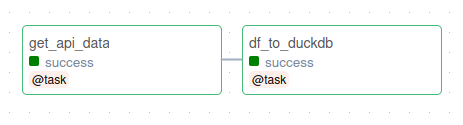
\includegraphics[width=0.8\textwidth, keepaspectratio]{img/[implem]airflow_dag.png} 
	\caption{Representación visual del flujo de tareas (DAG) en la interfaz de Apache Airflow.}
	\label{fig:airflow_dag}
\end{figure}

El flujo se configura para ejecutarse de manera autónoma con una periodicidad cronológica mediante el parámetro \texttt{schedule='*/15 * * * *'}, disparando una nueva ejecución de extracción, transformación y carga cada 15 minutos. El parámetro \texttt{catchup=False} asegura que, en caso de una caída del servidor, Airflow no intente ejecutar retrospectivamente todos los intervalos perdidos de forma simultánea, evitando así una violación de las políticas de uso de la API por exceso de peticiones.






\section{Despliegue en Producción}
\label{sec:despliegue_automatizacion}

En esta sección se detalla el proceso de empaquetado, configuración y despliegue del \textit{pipeline} ETL en un entorno de servidor remoto. La transición desde un entorno de desarrollo local hacia una infraestructura de producción resulta indispensable para garantizar la alta disponibilidad del sistema y la ingesta ininterrumpida de datos. 

\subsection{Arquitectura del sistema en Docker}
\label{subsec:arquitectura_docker}
Como se comenta anteriormente, para asegurar que los procesos de recolección de datos asíncronos operen sin interrupciones, el sistema se despliega en un servidor remoto. El acceso y desarrollo sobre este servidor se realiza mediante el protocolo \textit{Secure Shell} (SSH) a través del entorno de Visual Studio Code. 

Con el fin de evitar problemas de incompatibilidad de entornos, se opta por una arquitectura basada en contenedores utilizando \textit{Docker} y \textit{Docker Compose}. Se empaqueta el código junto con sus dependencias para garantizar que el sistema sea reproducible en cualquier servidor operativo, independientemente de su configuración base.

En relación con la configuración de Apache Airflow, se realiza una adaptación de la infraestructura oficial a las necesidades y recursos específicos del proyecto:
\begin{itemize}
	\item \textbf{Construcción de imagen personalizada.} Durante las pruebas de despliegue, la instalación dinámica de dependencias ha presentado conflictos de permisos al requerir compiladores del sistema (como \texttt{g++} para la compilación nativa de DuckDB). Para solventarlo, se diseña un \texttt{Dockerfile} propio que parte de la imagen base de Airflow: se instalan las herramientas del sistema operativo como superusuario (\texttt{root}) y, posteriormente, las librerías de Python de forma segura.
	\item \textbf{Mapeo de Volúmenes.} Se mapean los directorios locales del repositorio hacia el interior del contenedor. El directorio de código fuente se enruta a \texttt{/opt/airflow/plugins/src}, la base de datos DuckDB a \texttt{/opt/airflow/duck\_db}, y el archivo orquestador (\texttt{dag.py}) a la carpeta oficial \texttt{/opt/airflow/dags/} para su detección automática por el planificador.
	\item \textbf{Control de ejecución (\texttt{.airflowignore}).} Para evitar que el servidor web de Airflow procese código ajeno a la orquestación, se implementa un archivo \texttt{.airflowignore}. Esto restringe el escaneo a los módulos pertinentes para garantizar la estabilidad del contenedor.
\end{itemize}

Por otro lado, la monitorización del \textit{pipeline} requiere acceso a la interfaz gráfica (UI) de Airflow, la cual opera por defecto en el puerto 8080. Para maximizar la seguridad de la infraestructura y mitigar posibles vulnerabilidades, se decide no exponer dicho puerto en el \textit{firewall} público del servidor remoto. En su lugar, se implementa una estrategia de acceso mediante \textit{Port Forwarding} a través del túnel SSH. De este modo, se enruta el tráfico de red de forma cifrada desde el servidor hasta la máquina local.

\subsection{Lanzamiento y Monitorización}
\label{subsec:despliegue_docker}
Una vez configurados los parámetros del contenedor, el despliegue se inicializa mediante el comando \texttt{docker compose up -d}. La utilización del modo \textit{detached} permite que los servicios subyacentes de Airflow (planificador, servidor web, \textit{workers} y base de datos interna) se ejecuten en segundo plano.

Como resultado de este despliegue, el planificador de Airflow asume el control del ciclo de vida del \textit{pipeline}. En la Figura \ref{fig:airflow_grid} se presenta el historial de monitorización del sistema en producción, de forma que se evidencia la estabilidad de la ingesta recurrente cada 15 minutos sin intervención manual.

\begin{figure}[htbp]
	\centering
	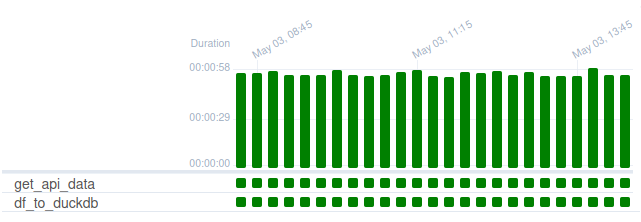
\includegraphics[width=0.9\textwidth, keepaspectratio]{img/[implem]airflow_grid.png} 
	\caption{Monitorización de las ejecuciones recurrentes del \textit{pipeline} ETL en el entorno de producción.}
	\label{fig:airflow_grid}
\end{figure}


\subsection{Finalización de la ingesta y consolidación de datos}
\label{subsec:finalizacion_etl}
Tras mantener el consumo de datos de forma ininterrumpida durante un mes, rango temporal suficiente para poder probar los modelos ya entrenados, se procede a la interrupción deliberada del sistema. Para garantizar la integridad de la base de datos y evitar problemas en el archivo físico, el proceso de desconexión se ejecuta en tres fases secuenciales:
\begin{enumerate}
	\item Se pausa la ejecución del grafo (DAG) directamente desde la interfaz gráfica de Apache Airflow, para evitar que el planificador dispare nuevas peticiones HTTP asíncronas a la API de Melbourne.
	\item Se detienen y destruyen los contenedores del servidor para asegurar un cierre limpio del motor de base de datos interno.
	\item Se realiza una copia de seguridad del archivo físico desde el servidor remoto hacia la máquina local, mediante protocolos de transferencia segura sobre el túnel SSH establecido.
\end{enumerate}




\section{Transformación del conjunto de datos en tiempo real}
\label{sec:procesamiento_oot}

Una vez consolidado el archivo físico de la base de datos en el entorno local, resulta imperativo transformar los registros crudos obtenidos de la API para que coincidan de forma exacta con la topología tensorial exigida por los modelos neuronales entrenados. El desafío técnico principal de esta fase radica en la naturaleza operativa de las APIs de los dispositivos emisores IoT, debido a que estos sistemas no emiten datos en un flujo constante, sino que se rigen por una arquitectura \textit{event-driven}: si el estado físico de una plaza no varía durante un periodo prolongado, el sistema no genera nuevas observaciones.

Este comportamiento es característico de las series temporales basadas en eventos, en las que la dinámica subyacente del sistema es continua, pero la observación es esparsa y dependiente de los cambios de estado \cite{event_based_iot}. En consecuencia, la aplicación directa de modelos de aprendizaje profundo exige la construcción de una representación temporal regular mediante técnicas de re-muestreo.

\subsection{Análisis estadístico de la dinámica temporal del sistema}
\label{subsec:eda_temporal}

Con el objetivo de caracterizar esta naturaleza esparsa, se realiza un análisis exploratorio de la distribución de los intervalos entre eventos consecutivos por sensor. Este análisis permite evaluar la regularidad del flujo de datos y cuantificar la presencia de interrupciones en la transmisión de la información.

Los resultados demuestran que la mediana de los intervalos entre eventos se sitúa en el orden de minutos, mientras que el percentil 95 se encuentra en torno a varias horas, lo cual se alinea con la rotación habitual de vehículos en un entorno urbano. No obstante, se observan casos en la cola de la distribución temporal que presentan intervalos de varios días de duranción e incluso semanas. Al no disponer de etiquetas explícitas de fallo emitidas por el sistema central, resulta matemáticamente imposible distinguir de forma determinista entre la inmovilidad prolongada de un vehículo y un fallo del dispositivo. Consecuentemente, la aplicación de cualquier umbral estricto basado en la duración del intervalo para la detección de sensores defectuosos introduciría supuestos empíricos no verificables y potencialmente sesgados. Por este motivo, el presente trabajo descarta la inferencia explícita de fallos a partir del truncamiento de la distribución de intervalos temporales.

\subsection{Procesamiento y reconstrucción de las señales}
\label{subsec:ffill_sota}

Para resolver la disparidad estructural y generar la matriz densa requerida por las redes neuronales, en primer lugar se eliminan los eventos duplicados y se genera un vector de tiempo continuo con una frecuencia estricta de 15 minutos, de forma análoga al proceso detallado en la sección \ref{subsec:procesamiento_pypots}. Al reindexar el conjunto de datos original sobre esta nueva cuadrícula homogénea, se generan vacíos explícitos en los intervalos sin eventos. 

Dado que el estado de ocupación de una plaza de aparcamiento presenta una alta propiedad de persistencia temporal, se adopta la hipótesis de \textit{Zero-Order Hold} (ZOH), ampliamente utilizada en sistemas dinámicos y procesamiento de señales telemáticas \cite{zero_order_hold_astrom}. Según este principio, el último estado observado se mantiene constante y válido hasta la llegada de una nueva observación que certifique lo contrario. Bajo este supuesto, los huecos generados tras el re-muestreo son reconstruidos íntegramente mediante un proceso de \textit{forward fill}.

Una vez completada la matriz continua, el proceso de estructuración tensorial y enriquecimiento trigonométrico es matemáticamente idéntico al desarrollado para el conjunto de datos histórico (véase la sección \ref{sec:data_preparation}), así como la técnica de ventanas deslizantes aplicada. No obstante, se deshabilita la generación de diferentes particiones, pues todos los datos se emplean en el mismo conjunto de \textit{test}. 

Se adoptan las dos aproximaciones homólogas diseñadas en el marco experimental previo:

\begin{enumerate}
	\item \textbf{Evaluación de imputación:} se evalúa mediante el mismo esquema de ausencia artificial (MCAR) descrito en la Sección \ref{sec:data_preparation}. Sobre la serie temporal previamente completada mediante ZOH, se enmascara de forma estocástica una proporción idéntica de las observaciones (e.g., 15\%). Esta inyección de ruido permite evaluar la capacidad de reconstrucción del modelo frente a caídas de red bajo escenarios donde existe un \textit{ground truth} absoluto \cite{du2023saits}.
	
	\item \textbf{Evaluación de predicción futura:} se ejecuta directamente sobre la serie temporal reconstruida mediante \textit{forward filling}, sin enmascaramiento.
\end{enumerate}




%%%%%%%%%%%%%%%%%%%%%%%%%%%%%%%%%%%%%%%%%%%%%%%%%%%%%%%%%%%%%%%%%%%%%%%%%%%%%%%%%%%%%%%%%%%%%%%%%%%%%%%%%
%%%%%%%%%%%%%%%%%%%%%%%%%%%%%%%%%%%%%%%%%%%%%%%%%%%%%%%%%%%%%%%%%%%%%%%%%%%%%%%%%%%%%%%%%%%%%%%%%%%%%%%%%
%%%%%%%%%%%%%%%%%%%%%%%%%%%%%%%%%%%%%%%%%%%%%%%%%%%%%%%%%%%%%%%%%%%%%%%%%%%%%%%%%%%%%%%%%%%%%%%%%%%%%%%%%
\section{Clasificación espacial de zonas de estacionamiento}
\label{sec:clasificacion_espacial}

La dinámica de ocupación y rotación de los estacionamientos urbanos está intrínsecamente ligada al entorno geográfico que los rodea. Dotar a cada sensor de un contexto espacial adicional, de forma complementaria a las coordenadas geográficas, simplifica la comprensión sobre cómo fluctua la demanda de los mismos. En consecuencia, se ha desarrollado un módulo específico encargado de clasificar el entorno urbano de cada plaza de aparcamiento y de generar una representación visual interactiva.


\subsection{Extracción de puntos de interés (POIs)}
\label{subsec:extraccion_pois}

Para determinar la naturaleza urbana del entorno de cada sensor, se utiliza la librería \texttt{OSMnx}, la cual permite interactuar directamente con la API pública de \textit{OpenStreetMap} (Overpass API). El flujo de ejecución parte de la lectura del conjunto de datos geolocalizados, generado previamente durante la fase del EDA tras el cruce del histórico con el inventario geoespacial de la ciudad.

Para cada sensor, el algoritmo delimita un radio de búsqueda estricto de 100 metros. Esta distancia se ha calibrado para capturar únicamente la calle e inmediaciones directas del aparcamiento, evitando sesgos por calles colindantes de diferente naturaleza. Dentro de este radio, se extraen y contabilizan elementos clave de la infraestructura urbana filtrando por etiquetas específicas (\textit{tags}): instalaciones públicas (\textit{amenities}), tiendas (\textit{shops}), oficinas (\textit{offices}) y tipología de edificios (\textit{building: residential, apartments}). 

Para garantizar la estabilidad del proceso y respetar los límites de la API pública, se implementa una estrategia de uso de memoria caché local y pausas controladas (\textit{rate limiting}) en las peticiones.

\subsection{Algoritmo de clasificación ponderada}
\label{subsec:clasificacion_ponderada}

El principal reto técnico en la clasificación espacial es la existencia de zonas de uso mixto, especialmente en el centro de la ciudad (\textit{Hoddle Grid} de Melbourne). En esta zona conviven rascacielos de oficinas, bajos comerciales y bloques de apartamentos residenciales. 

Para solucionarlo, se implementa un sistema de puntuación ponderada. El algoritmo asigna un peso matemático a cada elemento geográfico en función de su impacto en el tráfico urbano. Definimos las variables correspondientes al recuento de puntos de interés en el radio de búsqueda como: \(O\) (oficinas), \(S\) (comercios minoristas o \textit{shops}), \(A\) (instalaciones genéricas o \textit{amenities}) y \(R\) (edificios residenciales).

Con base en estas variables, se computan dos métricas o cargas principales:

\begin{itemize}
	\item \textbf{Carga Comercial (\(C_c\)):} otorga un peso alto a las oficinas debido a la gran afluencia diaria de trabajadores, un peso medio a los comercios minoristas y un peso unitario a las instalaciones genéricas.
	\begin{equation}
		\label{eq:carga_comercial}
		C_c = 5O + 3S + A
	\end{equation}
	
	\item \textbf{Carga Residencial (\(C_r\)):} asume que un solo polígono clasificado como edificio residencial alberga múltiples viviendas individuales, por lo que se le aplica un factor multiplicador elevado.
	\begin{equation}
		\label{eq:carga_residencial}
		C_r = 10R
	\end{equation}
\end{itemize}

Posteriormente, el algoritmo evalúa y compara ambas cargas mediante una función definida a tramos para establecer la categoría espacial dominante (\(Z\)) de la vía:

\begin{equation}
	\label{eq:clasificacion_zona}
	Z = 
	\begin{cases} 
		\text{\textit{Center (CBD)}}, & \text{si } C_c > 120 \lor O \geq 10 \\ 
		\text{\textit{Commercial}}, & \text{si } (C_c > C_r \land C_c > 20) \lor C_c > 10 \\ 
		\text{\textit{Residential}}, & \text{si } C_r > C_c \land R > 0 \\ 
		\text{\textit{General}}, & \text{en cualquier otro caso} 
	\end{cases}
\end{equation}

Esta formulación permite que si la carga comercial es extrema o supera un umbral crítico de densidad de oficinas, la zona se clasifique inequívocamente como centro financiero. Si existe competencia entre ambos usos, se impone la carga dominante, dejando la etiqueta \textit{General} como \textit{fallback} para zonas de baja densidad. Finalmente, todos los sensores clasificados se registran en un log de control (\texttt{pois\_sensors.log}) para facilitar su posterior auditoría y seguimiento.

\subsection{Renderizado cartográfico e integración Web}
\label{subsec:renderizado_mapa}

Una vez enriquecido el conjunto de datos con la nueva categorización espacial, la última etapa del flujo consiste en su representación gráfica mediante la librería \texttt{Folium}. 

Para maximizar el contraste visual de las distintas zonas, el mapa se inicializa centrado en las coordenadas del CBD de Melbourne empleando el mosaico oscuro \textit{CartoDB dark\_matter}. El algoritmo itera sobre el conjunto de sensores clasificados, proyectando un marcador circular sobre el plano para cada uno de ellos. A cada categoría urbana se le ha asignado un código de color específico, tal y como se ilustra en la Figura \ref{fig:folium_map}. Además, la visualización incorpora una leyenda descriptiva fijada mediante elementos HTML personalizados y un sistema de \textit{tooltips} interactivos. 

\begin{figure}
	\centering
	
\includegraphics[width=14cm, keepaspectratio]{[implem]folium_map.png}
	\caption{Distribución geográfica de las plazas de aparcamiento en Melbourne según su tipología urbana.}
	\label{fig:folium_map}
\end{figure}

Por otro lado, al posicionar el cursor sobre un sensor específico, la interfaz revela en tiempo real su identificador único, el nombre de la vía a la que pertenece y la clasificación espacial que el algoritmo le ha asignado. Se puede apreciar esta funcionalidad en la Figura \ref{fig:folium_sensor_hover}, 

\begin{figure}
	\centering
	
\includegraphics[width=7cm, keepaspectratio]{[implem]folium_hover.png}
	\caption{Detalle de la interfaz interactiva (\textit{tooltip}) al inspeccionar un sensor individual.}
	\label{fig:folium_sensor_hover}
\end{figure}

Finalmente, este mapa interactivo se exporta en formato HTML puro. Esta arquitectura de exportación permite que el mapa sea embebido de forma directa y fluida dentro de la página web documental del proyecto generada mediante \textbf{Quarto} sin requerir la ejecución local del código.





%%%%%%%%%%%%%%%%%%%%%%%%%%%%%%%%%%%%%%%%%%%%%%%%%%%%%%%%%%%%%%%%%%%%%%%%%%%%%%%%%%%%%%%%%%%%%%%%%%%%%%%%%
%%%%%%%%%%%%%%%%%%%%%%%%%%%%%%%%%%%%%%%%%%%%%%%%%%%%%%%%%%%%%%%%%%%%%%%%%%%%%%%%%%%%%%%%%%%%%%%%%%%%%%%%%
%%%%%%%%%%%%%%%%%%%%%%%%%%%%%%%%%%%%%%%%%%%%%%%%%%%%%%%%%%%%%%%%%%%%%%%%%%%%%%%%%%%%%%%%%%%%%%%%%%%%%%%%%
%%%%%%%%%%%%%%%%%%%%%%%%%%%%%%%%%%%%%%%%%%%%%%%%%%%%%%%%%%%%%%%%%%%%%%%%%%%%%%%%%%%%%%%%%%%%%%%%%%%%%%%%%
%%%%%%%%%%%%%%%%%%%%%%%%%%%%%%%%%%%%%%%%%%%%%%%%%%%%%%%%%%%%%%%%%%%%%%%%%%%%%%%%%%%%%%%%%%%%%%%%%%%%%%%%%
%%%%%%%%%%%%%%%%%%%%%%%%%%%%%%%%%%%%%%%%%%%%%%%%%%%%%%%%%%%%%%%%%%%%%%%%%%%%%%%%%%%%%%%%%%%%%%%%%%%%%%%%%
%%%%%%%%%%%%%%%%%%%%%%%%%%%%%%%%%%%%%%%%%%%%%%%%%%%%%%%%%%%%%%%%%%%%%%%%%%%%%%%%%%%%%%%%%%%%%%%%%%%%%%%%%
%%%%%%%%%%%%%%%%%%%%%%%%%%%%%%%%%%%%%%%%%%%%%%%%%%%%%%%%%%%%%%%%%%%%%%%%%%%%%%%%%%%%%%%%%%%%%%%%%%%%%%%%%
%%%%%%%%%%%%%%%%%%%%%%%%%%%%%%%%%%%%%%%%%%%%%%%%%%%%%%%%%%%%%%%%%%%%%%%%%%%%%%%%%%%%%%%%%%%%%%%%%%%%%%%%%

\section{Desarrollo del portal de resultados con Quarto}
\label{sec:portal_quarto}

Como culminación del flujo de procesamiento y modelado, se ha desarrollado un portal web interactivo destinado a la divulgación de los resultados del proyecto. Este entorno, construido íntegramente mediante el marco de publicación científica Quarto, permite trasladar la complejidad técnica del \textit{pipeline} de datos y de las redes neuronales a un formato accesible, navegable y visualmente atractivo.

\subsection{Configuración}
\label{subsec:quarto_config}

La orquestación del portal se gestiona a través de un archivo de configuración centralizado (\texttt{\_quarto.yml}). Se ha seleccionado una arquitectura de sitio web (\texttt{type: website}) renderizada en formato HTML5. Para el diseño de la interfaz de usuario (UI), se ha implementado el tema \textit{Cosmo}, el cual proporciona una estética limpia y minimalista, complementada con hojas de estilo personalizadas (\texttt{styles.css}).

Para optimizar la experiencia de usuario (UX) y la legibilidad de un proyecto con alta carga de programación, se han activado dos características fundamentales a nivel global:
\begin{itemize}
	\item \textbf{Índice de navegación dinámico (\texttt{toc: true}).} Genera automáticamente un menú lateral basado en la jerarquía de encabezados, facilitando el salto rápido entre secciones analíticas.
	\item \textbf{Plegado de código (\texttt{code-fold: true}).} Permite mantener una interfaz limpia al ocultar por defecto los bloques de código fuente (como los \textit{scripts} de Python) a la vez que ofrece al usuario la opción de desplegarlos interactuando con la interfaz si desea auditar la lógica subyacente.
\end{itemize}

\subsection{Navegación}
\label{subsec:quarto_estructura}

El contenido del portal se ha estructurado jerárquicamente a través de una barra de navegación principal (\textit{Navbar}), segmentando el proyecto en tres áreas clave de conocimiento:

\begin{enumerate}
	\item \textbf{Inicio (\texttt{index.qmd}).} Actúa como página de aterrizaje (\textit{landing page}) del proyecto. Presenta el contexto institucional mediante la inclusión gráfica del logotipo de la universidad, define el problema de la congestión del tráfico de agitación en Melbourne y resume la arquitectura metodológica en cuatro fases clave: ingesta analítica en DuckDB, procesamiento de series temporales, modelado mediante \textit{Deep Learning} (PyPOTS) y divulgación.
	\item \textbf{Visualizaciones (\texttt{visualizations.qmd}).} Espacio destinado a los resultados del Análisis Exploratorio de Datos (EDA) espacial y temporal. En esta sección se exponen los patrones descubiertos, integrando representaciones estáticas (como la detección de áreas de alta demanda o \textit{hotspots}) y mapas interactivos generados con Folium.
	\item \textbf{Resultados y Predicciones (\texttt{predictions.qmd}).} El núcleo evaluativo del modelo, donde se contrasta empíricamente el rendimiento de la red neuronal frente al \textit{ground truth} de los sensores.
\end{enumerate}

\subsection{Ejecución Dinámica y Representación Gráfica}
\label{subsec:quarto_dinamico}

El principal valor añadido de utilizar Quarto frente a un generador de sitios estáticos tradicional es su integración nativa con el motor de ejecución de \textit{Jupyter}. En lugar de importar imágenes estáticas pre-generadas, la página de resultados incluye bloques de código ejecutable que renderizan la información en el momento de la compilación del sitio.

A modo de ejemplo, para la evaluación visual del modelo PyPOTS, se embeben \textit{scripts} de Python utilizando la librería \texttt{Matplotlib}. Mediante directivas internas de Quarto (como \texttt{\#| label} y \texttt{\#| fig-cap}), el código procesa los tensores con la evolución horaria de la ocupación real medida por los sensores frente a los volúmenes predichos por la red neuronal, trazando comparativas dinámicas. 

Esta arquitectura asegura el paradigma de \textbf{investigación reproducible}: el documento final y el código que genera sus gráficos conviven en el mismo entorno fuente, garantizando que cualquier actualización en los pesos del modelo o en la base de datos DuckDB se refleje automáticamente en la web con una simple recompilación del proyecto.


